% Customisable fields and text areas start with % >> below.
% Lines starting with the comment character (%) are normally removed before release outside the collaboration, but not those 
% comments ending lines

% svn info. These are modified by svn at checkout time.
% The last version of these macros found before the maketitle will be the one on the front page,
% so only the main file is tracked.
% Do not edit by hand!
\RCS$Revision: 207461 $
\RCS$HeadURL: svn+ssh://dimatteo@svn.cern.ch/reps/tdr2/notes/IN-14-XXX/trunk/IN-14-XXX.tex$
\RCS$Id: IN-14-XXX.tex 207461 2013-09-18 14:56:50Z tapper $
%%%%%%%%%%%%% ptdr definitions %%%%%%%%%%%%%%%%%%%%%
%\input{ptdr-definitions} %These have been replaced by the equivalent style file
%%%%%%%%%%%%%%%  Title page %%%%%%%%%%%%%%%%%%%%%%%%
%%%%%%%%%%%%% local definitions %%%%%%%%%%%%%%%%%%%%%
% This allows for switching between one column and two column (cms@external) layouts
% The widths should  be modified for your particular figures. You'll need additional copies if you have more than one standard figure size.
\newlength\cmsFigWidth
\ifthenelse{\boolean{cms@external}}{\setlength\cmsFigWidth{0.85\columnwidth}}{\setlength\cmsFigWidth{0.4\textwidth}}
\ifthenelse{\boolean{cms@external}}{\providecommand{\cmsLeft}{top}}{\providecommand{\cmsLeft}{left}}
\ifthenelse{\boolean{cms@external}}{\providecommand{\cmsRight}{bottom}}{\providecommand{\cmsRight}{right}}
%%%%%%%%%%%%% local definitions %%%%%%%%%%%%%%%%%%%%%
\newcommand{\CLs}{\ensuremath{CL_\mathrm{s}}}
\newcommand{\CLb}{\ensuremath{CL_\mathrm{b}}}
\newcommand{\CLsb}{\ensuremath{CL_\mathrm{s+b}}}

%\newcommand{\GeV}{\ensuremath{\mathrm{Ge\kern -0.1em V}}}
%\newcommand{\TeV}{\ensuremath{\mathrm{Te\kern -0.1em V}}}
%\newcommand{\TeVcc}{\ensuremath{\,\mathrm{Te\kern -0.1em V\!/c}^2}}
%\newcommand{\GeVcc}{\ensuremath{\,\mathrm{Ge\kern -0.1em V\!/c}^2}}
%\newcommand{\MeVcc}{\ensuremath{\,\mathrm{Me\kern -0.1em V\!/c}^2}}
%\newcommand{\GeVc}{\ensuremath{\mathrm{Ge\kern -0.1em V}\!/c}}
%\newcommand{\nanob}{\mbox{{\rm ~nb}~}}
%\newcommand{\fb}{\ensuremath{\mathrm{fb}}}
%\newcommand{\pb}{\ensuremath{\mathrm{pb}}}
\newcommand{\ifb}{\ensuremath{\mathrm{fb^{-1}}}}
%\newcommand{\ipb}{\ensuremath{\mathrm{pb^{-1}}}}
%\newcommand{\grad}{\ensuremath{^{\circ}}}
%
% Special user made math symbols
%
%\newcommand{\lsim}{\raisebox{-1.5mm}{$\:\stackrel{\textstyle{<}}{\textstyle{\sim}}\:$}}
%\newcommand{\gsim}{\raisebox{-1.5mm}{$\:\stackrel{\textstyle{>}}{\textstyle{\sim}}\:$}}

% particles

\newcommand{\pipm}{\ensuremath{\pi^{\pm}}}
\newcommand{\pizero}{\ensuremath{\pi^{0}}}
\newcommand{\Hi}{\PH\xspace}
\newcommand{\V}{\ensuremath{\mathrm{V}}}
\newcommand{\W}{\PW}
\newcommand{\Wjets}{\ensuremath{\mathrm{W+jets}}}
\newcommand{\Zjets}{\ensuremath{\mathrm{Z+jets}}}
\newcommand{\Wt}{\ensuremath{\mathrm{Wt}}}
\newcommand{\Wstar}{\ensuremath{\mathrm{W}^{*}}}
\newcommand{\Wparenthesisstar}{\ensuremath{\mathrm{W}^{(*)}}}
\newcommand{\WW}{\PW\PW\xspace}
%\newcommand{\Z}{\ensuremath{\mathrm{Z}}}
\newcommand{\Zstar}{\ensuremath{\mathrm{Z}^{*}}}
\newcommand{\Astar}{\ensuremath{\mathrm{\gamma}^{*}}}
\newcommand{\ZZ}{\ensuremath{\Z\Z}}
\newcommand{\WZ}{\ensuremath{\W\Z}}
\newcommand{\VVV}{\ensuremath{\V\V\V}}
\newcommand{\Wgstar}{\ensuremath{\W\gamma}^{*}}
\newcommand{\E}{\Pe}
\newcommand{\Ep}{\Pep}
%\newcommand{\Em}{\ensuremath{\mathrm{e}^{-}}}
\newcommand{\Epm}{\ensuremath{\Pe^{\pm}}}
\newcommand{\Emp}{\ensuremath{\Pe^{\mp}}}
\newcommand{\M}{\Pgm}
\newcommand{\Mp}{\Pgmp}
\newcommand{\Mm}{\Pgmm}
\newcommand{\Mpm}{\ensuremath{\mu^{\pm}}}
\newcommand{\Mmp}{\ensuremath{\mu^{\mp}}}
\newcommand{\Tau}{\ensuremath{\tau}}
\newcommand{\Nu}{\ensuremath{\nu}}
\newcommand{\Nubar}{\ensuremath{\overline{\nu}}}
\newcommand{\Lep}{\ensuremath{\ell}}
\newcommand{\Lepp}{\ensuremath{\ell^{+}}}
\newcommand{\Lepm}{\ensuremath{\ell^{-}}}
\newcommand{\Lprime}{\ensuremath{\Lep^{\prime}}}
\newcommand{\Prot}{\Pp}
\newcommand{\Pbar}{\Pap}
\newcommand{\PP}{\Pp\Pp}
\newcommand{\PPbar}{\Pp\Pap}
%\newcommand{\ttbar}{\ensuremath{\mathrm{t}\bar{\mathrm{t}}}}
\newcommand{\qq}{\ensuremath{\mathrm{q}\mathrm{q}}}
\newcommand{\qqbar}{\ensuremath{\mathrm{q}\overline{\mathrm{q}}}}
\newcommand{\Wtb}{\ensuremath{\W\mathrm{t}\mathrm{b}}}
\newcommand{\Top}{\ensuremath{\mathrm{t}}}
\newcommand{\Bot}{\ensuremath{\mathrm{b}}}
\newcommand{\Atop}{\ensuremath{\overline{\mathrm{t}}}}
\newcommand{\Abot}{\ensuremath{\overline{\mathrm{b}}}}
% arrow
\newcommand{\To}{\ensuremath{\rightarrow}}

% masses
\newcommand{\mH}{\ensuremath{m_{\PH}}}
\newcommand{\mHi}{\ensuremath{m_{\PH}}\xspace}
\newcommand{\mW}{\ensuremath{m_{\PW}}}
\newcommand{\mZ}{\ensuremath{m_{\cPZ}}}
\newcommand{\mll}{\ensuremath{m_{\Lep\Lep}}}
\newcommand{\mt}{\ensuremath{m_{\mathrm{T}}}}
%%%\newcommand{\mth}{\ensuremath{m_{\mathrm{T}}^{\ell\ell\not{E}_{\mathrm T}}}}
\newcommand{\mth}{\ensuremath{m_{\mathrm{T}}}}
\newcommand{\mtlnjj}{\ensuremath{m_{\mathrm{T}}^{\ell\nu 2j}}}
\newcommand{\mr}{\ensuremath{m_{\mathrm{R}}}}
\newcommand{\delphir}{\ensuremath{\Delta\phi_{\mathrm{R}}}}

% generators
\newcommand{\pythia} {\textsc{pythia}}
\newcommand{\geant} {\textsc{geant4}}
\newcommand{\herwig} {\textsc{herwig}}
\newcommand{\acermc} {\textsc{acermc}}
\newcommand{\jimmy} {\textsc{jimmy}}
\newcommand{\mcatnlo} {\textsc{mc@nlo}}
\newcommand{\sherpa} {\textsc{sherpa}}
\newcommand{\madgraph} {\textsc{madgraph}}
\newcommand{\mcfm} {\textsc{mcfm}}
\newcommand{\powheg} {\textsc{powheg}}
\newcommand{\Phantom} {\textsc{phantom}}
\newcommand{\fastjet} {\textsc{fastJet}}
\newcommand{\tauola} {\textsc{tauola}}

% kinematics
% \newcommand{\pt}{\ensuremath{p_\mathrm{T}}}
\newcommand{\Et}{\ensuremath{E_\mathrm{T}}}
\newcommand{\ptveto}{\ensuremath{\pt^\text{veto}}}
\newcommand{\ptl}{\ensuremath{p_\perp^{\Lep}}}
\newcommand{\ptlmax}{\ensuremath{p_{\mathrm{T}}^{\Lep,\text{max}}}}
\newcommand{\ptlmin}{\ensuremath{p_{\mathrm{T}}^{\Lep,\text{min}}}}
\newcommand{\ptll}{\ensuremath{\pt^{\ell\ell}}}
\newcommand{\met}{\ensuremath{\Et^{\text{miss}}}}
\newcommand{\delphill}{\ensuremath{\Delta\phi_{\Lep\Lep}}}
\newcommand{\deletall}{\ensuremath{\Delta\eta_{\Lep\Lep}}}
\newcommand{\delphimetl}{\ensuremath{\Delta\phi(\vec{E}_\mathrm{T}^{\text{miss}},\Lep)}}
\newcommand{\delphillmet}{\ensuremath{\Delta\phi(\Lep\Lep,\vec{E}_\mathrm{T}^{\text{miss}})}}
\newcommand{\delR}{\ensuremath{\Delta R}}
\newcommand{\Eta}{\ensuremath{\eta}}
\newcommand{\GAMMA}{\ensuremath{\gamma}}
\newcommand{\pmet}{\ensuremath{E^{\text{miss}\angle}_\mathrm{T}}}
\newcommand{\vmet}{\ensuremath{\vec{E}_\mathrm{T}}^{\text{miss}}}

%efficiencies
\newcommand{\effsig}{\ensuremath{\varepsilon_{\text{bkg}}^{\mathrm{S}}}}
\newcommand{\effnorm}{\ensuremath{\varepsilon_{\text{bkg}}^{\mathrm{N}}}}
\newcommand{\Nsig}{\ensuremath{N_{\text{bkg}}^{\mathrm{S}}}}
\newcommand{\Nnorm}{\ensuremath{N_{\text{bkg}}^{\mathrm{N}}}}

% processes
\newcommand{\dyeepm}{\ensuremath{{\Z}/\GAMMA^*{\to \Pep\Pem}}}
\newcommand{\dymmpm}{\ensuremath{{\Z/}\GAMMA^*\to\Pgmp\Pgmm}}
\newcommand{\dyttpm}{\ensuremath{{\Z}/\GAMMA^* \to\tau^+\tau^-}}
\newcommand{\dyllpm}{\ensuremath{{\Z}/\GAMMA^*{\to \ell^+\ell^-}}}
\newcommand{\dyee}{\ensuremath{{\Z}/\GAMMA^*{\to \Pe\Pe}}}
\newcommand{\dymm}{\ensuremath{{\Z/}\GAMMA^*\to\mu\mu}}
\newcommand{\dytt}{\ensuremath{{\Z}/\GAMMA^* \to\tau\tau}}
\newcommand{\dyll}{\ensuremath{{\Z}/\GAMMA^*{\to \ell\ell}}}
\newcommand{\zee}{\ensuremath{{\Z\to \Pep\Pem}}}
\newcommand{\zmm}{\ensuremath{{\Z}\to\Pgmp\Pgmm}}
\newcommand{\ztt}{\ensuremath{{\Z}\to\tau^+\tau^-}}
\newcommand{\zll}{\ensuremath{{\Z\to \ell^+\ell^-}}}
\newcommand{\ppww}{\ensuremath{pp \to \PWp\PWm}}
\newcommand{\wwlnln}{\ensuremath{\PWp\PWm\to \ell^+\nu \ell^-\overline{\nu}}}
\newcommand{\ww}{\ensuremath{\W\W}}
\newcommand{\WWpm}{\ensuremath{\PWp\PWm}}
\newcommand{\Hww}{\Hi\to\WW}
\newcommand{\hww}{\Hi\to\WW}
\newcommand{\hwwnopm}{\Hi\to\ww}
\newcommand{\hwwlnlnnopm}{\ensuremath{\Hi\to \W\W\to \ell \nu \ell \nu}}
\newcommand{\wz}{{\PW\cPZ}}
\newcommand{\zz}{{\cPZ\cPZ}}
\newcommand{\wgamma}{\ensuremath{\W\GAMMA}}
\newcommand{\wjets}{\ensuremath{\PW+}\text{jets}}
\newcommand{\tw}{\ensuremath{\mathrm{t}\W}}
\newcommand{\singletopt}{\ensuremath{t} ($t$-chan)}
\newcommand{\singletops}{\ensuremath{t} ($s$-chan)}

%other
\def\fixme{({\bf FixMe})}
\newcommand{\ee}{\ensuremath{ee}}
\newcommand{\emu}{\ensuremath{e\mu}}
\def\mm{\ensuremath{\mu\mu}}
\newcommand{\spintwopmin}{\ensuremath{2^+_\text{min}}}

% integrated luminosity
\newcommand{\usedLumi}{19.7 \fbinv}
\newcommand{\usedLumiWithSyst}{\ensuremath{19.7 \pm 0.5 \fbinv}}

%%%%%%%%%%%%%%%  Title page %%%%%%%%%%%%%%%%%%%%%%%%
\cmsNoteHeader{IN 2014/XXX} % This is over-written in the CMS environment: useful as preprint no. for export versions
% >> Title: please make sure that the non-TeX equivalent is in PDFTitle below
\title{Dynamic Data Management for Tier-3 Sites}

% >> Authors
%Author is always "The CMS Collaboration" for PAS and papers, so author, etc, below will be ignored in those cases
%For multiple affiliations, create an address entry for the combination
\address[MIT]{Massachusetts Institute of Technology}

\author[MIT]{L. Di Matteo}
\author[MIT]{M. Goncharov}
\author[MIT]{J. Lawhorn}
\author[MIT]{C. Paus}

% >> Date
% The date is in yyyy/mm/dd format. Today has been
% redefined to match, but if the date needs to be fixed, please write it in this fashion.
% For papers and PAS, \today is taken as the date the head file (this one) was last modified according to svn: see the RCS Id string above.
% For the final version it is best to "touch" the head file to make sure it has the latest date.
\date{\today}

% >> Abstract
% Abstract processing:
% 1. **DO NOT use \include or \input** to include the abstract: our abstract extractor will not search through other files than this one.
% 2. **DO NOT use %**                  to comment out sections of the abstract: the extractor will still grab those lines (and they won't be comments any longer!).
% 3. **DO NOT use tex macros**         in the abstract: External TeX parsers used on the abstract don't understand them.
\abstract{
CMS data is ordered in datasets, which have some common properties and are usually
analyzed together. As data taking progresses and Monte Carlo tools improve, datasets are often
replaced and site administrators have to identify and delete out-dated datasets. In this note we 
document a novel approach to dataset managing aimed at the full automatization of the dataset ranking, 
deletion and download procedures. We focus on an implementation of this system at the computing 
facility T3\_US\_MIT.
}

% >> PDF Metadata
% Do not comment out the following hypersetup lines (metadata). They will disappear in NODRAFT mode and are needed by CDS.
% Also: make sure that the values of the metadata items are sensible. For APS submissions, they are automatically converted to APS keywords.
\hypersetup{%
pdfauthor={L. Di Matteo, M. Goncharov, J. Klawhorn, C. Paus},%
pdftitle={Dynamic Data Management for Tier-3 Sites},%
pdfsubject={CMS},%
pdfkeywords={CMS, trigger, jets, pile up}}

\maketitle %maketitle comes after all the front information has been supplied

\tableofcontents
% >> Text
%%%%%%%%%%%%%%%%%%%%%%%%%%%%%%%%  Begin text %%%%%%%%%%%%%%%%%%%%%%%%%%%%%
%% **DO NOT REMOVE THE BIBLIOGRAPHY** which is located before the appendix.
%% You can take the text between here and the bibiliography as an example which you should replace with the actual text of your document.
%% If you include other TeX files, be sure to use "\input{filename}" rather than "\input filename".
%% The latter works for you, but our parser looks for the braces and will break when uploading the document.
%%%%%%%%%%%%%%%

\section{Introduction}\label{sec:introduction}
The Large Hadron Collider (LHC) has been colliding protons at $\sqrt{s}=$7 TeV and 8 TeV from 2010 to end of 2012. 
This period is referred to as Run-I. The highlight of Run-I was the discovery of a new heavy particle at about 125 GeV, 
consistent with the long-sough Standard Model Higgs Boson~\cite{ATLASHiggs,CMSHiggs}. 

Currently, CMS has about 50 PB of datasets, corresponding to an integrated luminosity of 25 \fbinv. In order to identify 
the very few, rare events that are clear signatures of new physics in our detector, we must optimally use the available 
computing resources. The computing challenge will become harder with time, as the amount of collected data will increase 
substantially in the years to come. The schedule at present foresees two major data taking phases - Run-II and Run-III - 
which have the following characteristics (Run-I is also shown for comparison):

\begin{itemize}
	\item Run-I: 2010-2012, nominal collision energy 7(8) TeV, accumulated data \\ 50 PB (5(20) \fbinv); 
	\item Run-II: 2015-2017, nominal collision energy 13 TeV, accumulated data \\ 200 PB ($\sim$ 100 \fbinv); 
	\item Run-III: 2019-2021, nominal collision energy 14 TeV, accumulated data \\ 400 PB ($\sim$ 300 \fbinv). 
\end{itemize}
The numbers are staggering and while computing resources will grow and algorithmic adjustments will be made as well, it is 
obvious that an optimization of the present system is going to have a major impact on this endeavor.

CMS is now proposing to make best use of our computing resources by employing a novel way of managing the data distribution, based on a dynamic system that will be able to optimize the performance using a number of different system metrics.
The plan is to treat all CMS computing sites as a network of massive caches. The optimization of the CMS data distribution in these caches is a challenging task because the system contains order of 50 geographically separated computing centers of quite different properties, and the computing tasks to be performed on them cover a wide parameter space in terms of their computing requirements. Considering the complexity of the optimization problem with perfectly working components and further including component failures into the task it is clear that there is no analytic solution and machine learning algorithms seem a great candidate to achieve a reliable and - once properly trained - low maintenance solution.

While this is a long term project that is involving the large computing community of CMS, the MIT HEP computing group has been pioneering techniques to perform 
automated data management at our local facilities, and here we document the core functionalities of the system that we designed, 
translated into software, tested and put into production.


\section{The MIT HEP Computing System}\label{sec:mithepcomp}
The MIT High Energy Physics group, part of the MIT Particle Physics Collaboration (PPC), 
currently manages a large computing facility - T2\_US\_MIT - and a smaller computing cluster 
- T3\_US\_MIT - as part of the CMS computing system.

\subsection{The MIT HEP Tier-2}

The MIT HEP Tier-2 (T2\_US\_MIT), located in the MIT-Bates High Performance Research Computing 
Facility (HPRCF), currently hosts about 5000 cores and 3.5 PB of data. The site uplink
speed is 10 Gb/s.

The machines are organized into servers and worker nodes (WNs), which provide a mix of CPU and 
storage space. 

\subsection{The MIT HEP Tier-3}

The MIT HEP Tier-3 (T3\_US\_MIT) located on the MIT campus, currently hosts about 600
cores and 0.3 PB of data. The site uplink speed is 8 Gb/s.

Similar to the Tier-2, the machines are organized into servers and WNs, which provide a mix of CPU and storage 
space. In addition, a significant number of machines, characterized by low-end CPU and memory 
availability, are used as data transfer nodes (TNs).

In the current scheme, T3\_US\_MIT is used to test new services before deployment on the larger site, 
as the Tier-3 hosts only datasets owned by the MIT group, while Tier-2 hosts datasets shared among the 
CMS community, hence downtime and disservices at T2\_US\_MIT will affect a larger community of scientists.





\section{The MIT HEP Dynamic Data}\label{sec:mithepdd}
As already specified, CMS maintains a huge amount of data, O(50PB), organized 
in datasets, which share common properties and users tend to analyze as a whole. 
Datasets are further subdivided into data blocks consisting of one or more files. These 
subdivisions facilitate the handling of the datasets.

A convenient set of tools exists to move data around but there is no intelligent tool to produce and
distribute copies of popular data or automatically remove less popular data. At present the various 
physics groups each have a data manager who is responsible for disk management. Usually this involves 
the management of about three Tier-2 computing sites and about a thousand 
datasets (mostly Monte Carlo simulation). Placement of new data is relatively straight forward but the 
deletion of older sets can be quite complicated and requires significant amount of time.

At MIT, we have tried to tackle this problem by considering a small subset of the CMS computing system, 
i.e. the two sites sub-system \{T2\_US\_MIT,T3\_US\_MIT\}. In this sub-system we have the following:

\begin{itemize}
	\item all datasets relevant for MIT analyses are stored on the Tier-2;
	\item all data analysis jobs are run on Tier-3 machines;
	\item the available disk space of the Tier-3 is not enough to store all datasets necessary for 
	the completion of all the analyses.
	\item users typically re-run a given analysis workflow multiple times on the same group of datasets in 
	a relatively short timescale.
\end{itemize}
We have designed and implemented an automated service, the \textbf{MIT HEP Dynamic Data (MITHDD)}, that 
caches the datasets on Tier-3, using the Tier-2 as a source pool. 

MITHDD is divided into two subservices: \textbf{SmartCache}, which is responsible for transferring 
datasets from Tier-2 to Tier-3, and \textbf{Cinderella}, which is responsible for deletions on Tier-3.

The source code of MITHDD follows the same structure and is currently available on \textsc{GitHub} at 
\href{https://github.com/cpausmit/DynamicData}{\textcolor{Mahogany}{this link}}. The software is licensed
under \href{http://opensource.org/licenses/MIT}{\textcolor{Mahogany}{these terms}}.

\subsection{SmartCache}\label{subsec:smartcache}
The scope of SmartCache is to create and handle transfer requests needed to ensure that 
user jobs, running on Tier-3, can analyze datasets stored only on the Tier-2. Datasets are organized into 
files, which are mapped in the SmartCache \textsc{MySQL} database. These files are the fundamental blocks 
managed by SmartCache. A system daemon interfaces with the file database, and it periodically 
performs the following operations:

\begin{enumerate}
	\item collects dataset requests, if any, and checks which files are not stored on Tier-3;
	\item creates transfers requests for all files that need to be transferred on Tier-3;
	\item keeps track of pending transfers until they are completed;
	\item saves relevant information for each transfer (status, speed, ecc...);
	\item updates the file database.
\end{enumerate}

The daemon exploits the Tier-3 batch system to submit jobs for file transfers. The transfer technology 
is based on LCG Data Management Client Tools, supported by the OSG consortium~\cite{OSG1,OSG2}. The use of 
the batch system for downloads allows concurrent multiple file transfers, limited only by the number slots 
allocated for this particular service. This model is particularly interesting as it can be scaled with minimal 
effort, since the allocation and management of the batch system slots is performed with standard cluster 
tools (in the case of our site \textsc{HTCondor}).

\subsubsection{SmartCache Monitoring}

We have also designed and implemented a system that periodically checks the status of SmartCache, analyzes it
and produces plots in order to track the performance of our caching system.

The monitoring tool computes and plots the following distributions:

\begin{itemize}
	\item \textbf{SmartCache transfer rate}, which shows the cumulative transfer speed for the caching jobs at
	any given time;
	\item \textbf{SmartCache transfer failures}, i.e. the rate of failed transfers as a function of time;
	\item \textbf{Lag time}, which shows the time lapse between the file download request and the start of the file transfer;
	\item \textbf{Speed}, i.e. the file transfer rate (not cumulative).
\end{itemize}

These distributions are computed for five different time periods - last hour, last day, last week, last month, all times - 
and are uploaded to the web and available at 
\href{http://t3serv001.mit.edu/~paus/plots/}{\textcolor{Mahogany}{this link}}.

As an example of the monitoring output, we report in Figure~\ref{fig:SmartCache} the summary plots for the month of
August 2014. 

\begin{figure}[htbp]
 \centering
 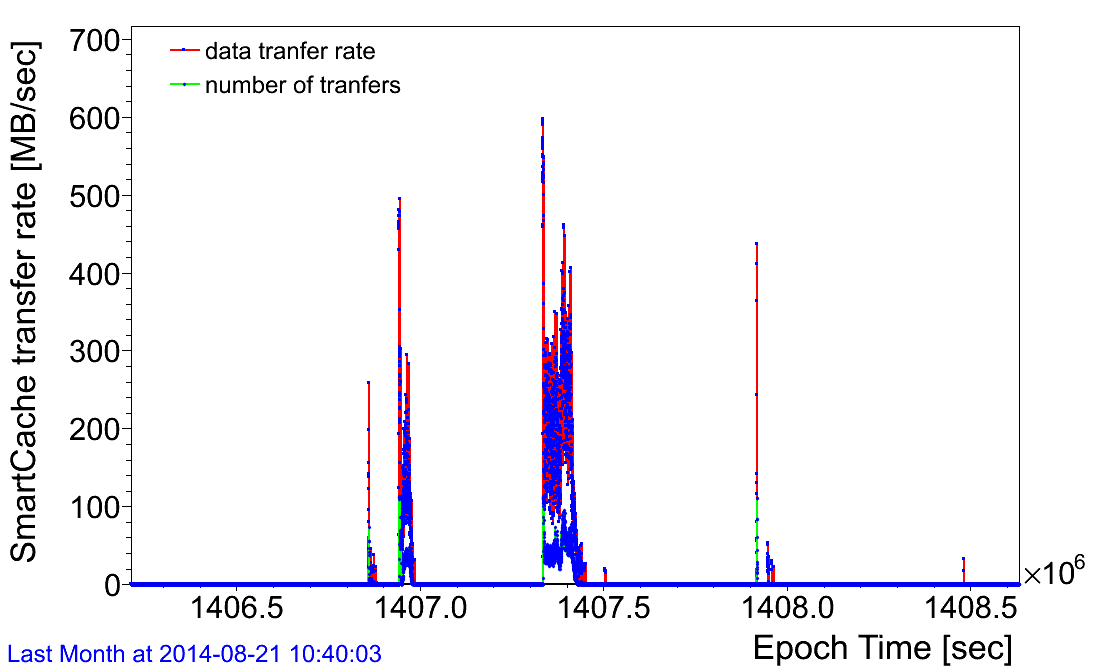
\includegraphics[angle=0,width=0.49\textwidth]{plots/transferRateLastMonth.png}
 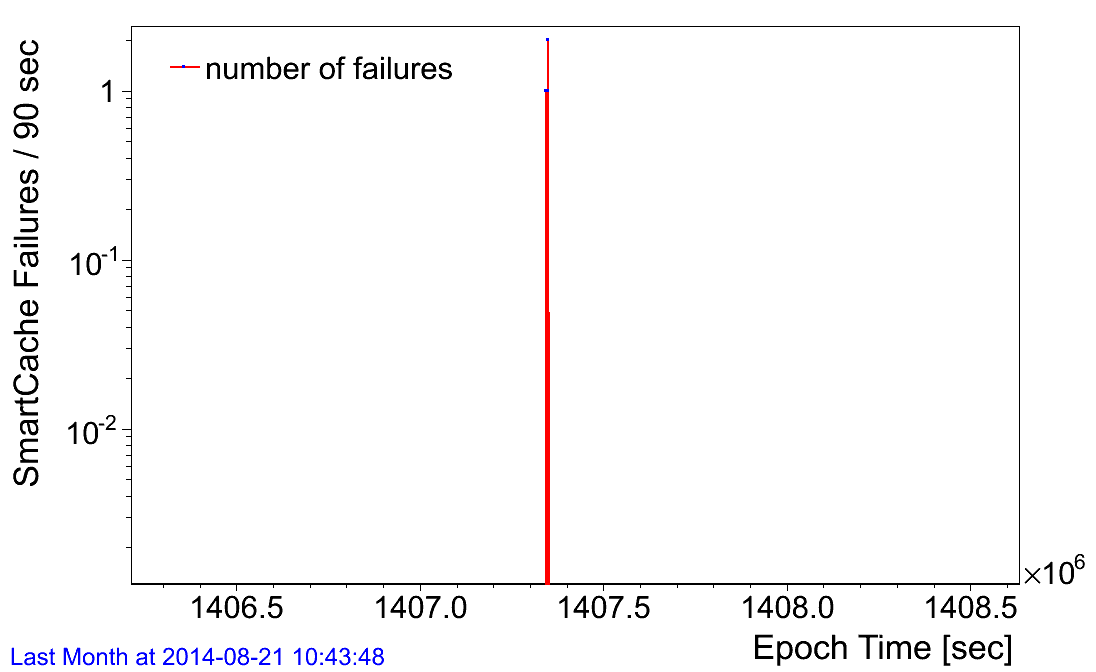
\includegraphics[angle=0,width=0.49\textwidth]{plots/failuresLastMonth.png}
 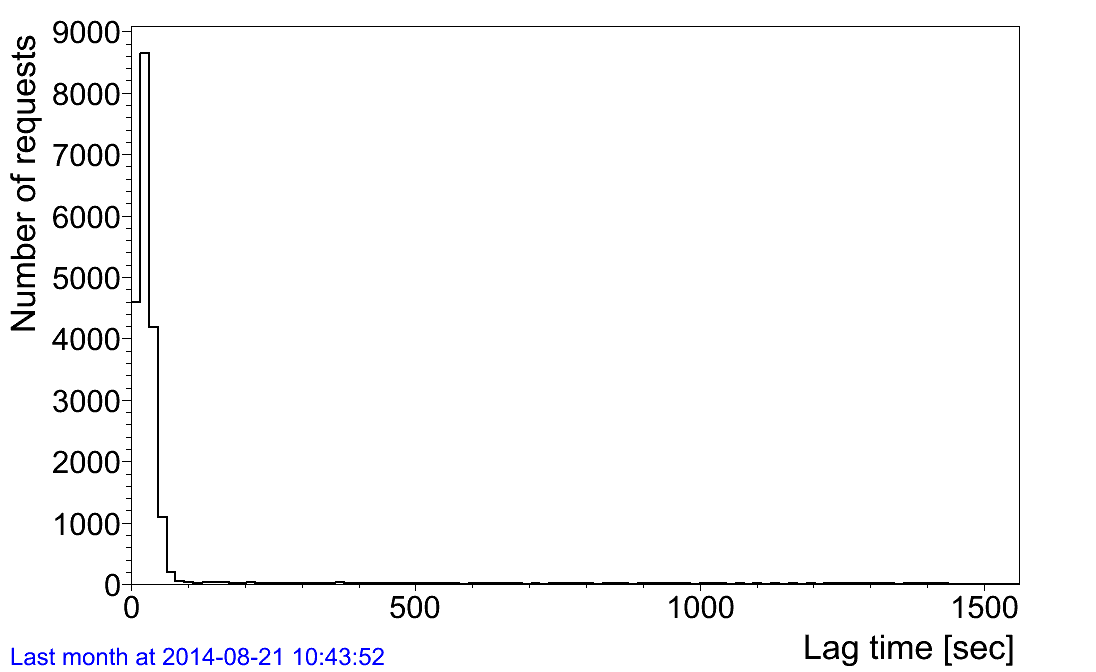
\includegraphics[angle=0,width=0.49\textwidth]{plots/lagTimeLastMonth.png}
 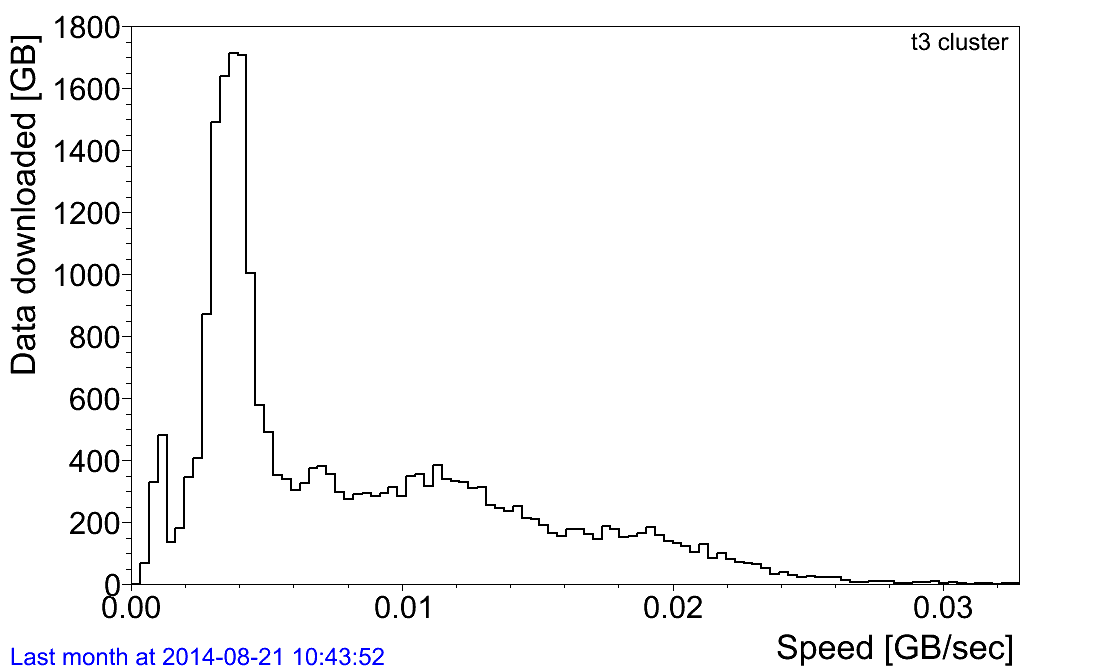
\includegraphics[angle=0,width=0.49\textwidth]{plots/downloadSpeedLastMonth.png}
 \caption{SmartCache monitoring plots for the month of August 2014. In the figures, from top row to bottom row, left to right,
 SmartCache transfer rate, SmartCache transfer failures, Lag time and Speed.}
 \label{fig:SmartCache}
\end{figure}

For of our site, it is interesting to look at Figure~\ref{fig:SmartCache} top-left. First of all it 
shows that we can cache datasets at a total speed of about 5 Gb/s. In addition, we could possibly improve this by
adding more machines to our cacher pool:
at T3\_US\_MIT there are currently 33 machines dedicated to transfers, each carrying an average of three slots, 
thus up to about 100 transfers can happen. Even considering the bandwidth limitation of each machine, we would expect
to be able to saturate our uplink speed, i.e. 8 Gb/s. Nevertheless, the
rate plot shows that the maximum caching speed saturates at 60\% of the total available bandwidth.
Thus, we are limited by some non-network related factors (likely the disk writing speed on TNs).


\subsection{Cinderella}\label{subsec:cinderella}
The design of Cinderella follows the requirements of an automatic cache release process needed for the 
CMS computing. This cache release process is supposed to optimize the usage of all 
available disk storage and relieve the data managers of a large fraction of their work by:

\begin{enumerate}
	\item keeping all storage filled to a high and safe level;
	\item always allow new data to be received at any site;
	\item remove the least valuable data from the storage when the storage fills over a given level.
\end{enumerate}

In order to perform a cache release, the system is periodically reviewed to ensure there is free space 
for transfers at the site. The condition for the cache release is given by:

\begin{itemize}
	\item usedSpace / availableSpace $>$ 92\% (number can be adjusted);
\end{itemize}

When the cache release algorithm is triggered, enough datasets to restore the target free space are identified
for deletion in order to fulfill the following condition:

\begin{itemize}
	\item usedSpace / availableSpace $<$ 87\% (number can be adjusted);
\end{itemize}

To select datasets for deletion we algorithmically rank all datasets. We select datasets with the lowest priority
by adding the space they occupy until we have enough space to meet the above condition. The selected datasets are 
then removed from storage. The ranking algorithm evaluates the usefulness of the data. For our site, the ranking 
algorithm uses only the time of latest access, such that the lowest priority datasets were accessed longest ago. 

Cinderella implements the algorithm described above. The core parts of the software are
a \textsc{MySQL} database, which stores the list of datasets and relevant information needed to generate the ranking
and perform the cache release, and a daemon that periodically checks if the release trigger condition is met.
In case of a triggered release, the Cinderella daemon issues the deletion command and updates the dataset database.

The Cinderella service also takes periodic snapshots of the dataset database, and uploads them online at 
\href{http://t3serv001.mit.edu/~cmsprod/dynamicdata/cinderella.html}{\textcolor{Mahogany}{this webpage}}.
The snapshots show a ranked list of datasets in our database according to the algorithm used for the
cache release. For each dataset, the number of accesses, number of downloads, caching status (which 
determines if that dataset is present on the Tier-3 cache), last access time and size are listed.
In the current color scheme, blue denotes datasets that were at some point cached but have been deleted and
are not currently stored in cache, red shows the list of datasets that will be deleted in case the cache release
condition is met, and black shows the remaining datasets.

During 6 months of operations, Cinderella has been responsible for deletions that amount to a total of 0.1 PB
of disk space, equivalent to 1/3 of the entire Tier-3 storage capabilities. Equivalently, the system has 
triggered a cache release about ten times.









\section{Summary}
The amount of resources needed for the CMS computing system will grow significantly as we are approaching the 
beginning of LHC Run-II, and the CMS computing management is now proposing to make best use of our infrastructure by employing a 
novel way of managing the data distribution.

In this document, we have summarized the fundamental ingredients of the new Dynamic Data Management system, in particular
we have focused on the MIT HEP computing resources, where a simplified prototype of such a system has been already set in place.

We have introduced the MIT HEP Dynamic Data, and summarized its core structure, functionalities and scope.
Examples of the good performances of our system have been reported, as well as live pages where any user can access and 
evaluate our product. 

Our experience with this new way of data managing is overall extremely positive and we think that other sites might as well 
benefit from it, and eventually that this will lead to an improved usage of the CMS computing resources.

% >> acknowledgements (for journal papers)
% Please include the latest version from https://twiki.cern.ch/twiki/bin/viewauth/CMS/Internal/PubAcknow.
\section*{Acknowledgements}
We congratulate our colleagues in the CERN accelerator departments for the excellent performance of the LHC and thank the technical and administrative staffs at CERN and at other CMS institutes for their contributions to the success of the CMS effort. In addition, we gratefully acknowledge the computing centres and personnel of the Worldwide LHC Computing Grid for delivering so effectively the computing infrastructure essential to our analyses. Finally, we acknowledge the enduring support for the construction and operation of the LHC and the CMS detector provided by the following funding agencies: BMWFW and FWF (Austria); FNRS and FWO (Belgium); CNPq, CAPES, FAPERJ, and FAPESP (Brazil); MES (Bulgaria); CERN; CAS, MoST, and NSFC (China); COLCIENCIAS (Colombia); MSES and CSF (Croatia); RPF (Cyprus); MoER, ERC IUT and ERDF (Estonia); Academy of Finland, MEC, and HIP (Finland); CEA and CNRS/IN2P3 (France); BMBF, DFG, and HGF (Germany); GSRT (Greece); OTKA and NIH (Hungary); DAE and DST (India); IPM (Iran); SFI (Ireland); INFN (Italy); NRF and WCU (Republic of Korea); LAS (Lithuania); MOE and UM (Malaysia); CINVESTAV, CONACYT, SEP, and UASLP-FAI (Mexico); MBIE (New Zealand); PAEC (Pakistan); MSHE and NSC (Poland); FCT (Portugal); JINR (Dubna); MON, RosAtom, RAS and RFBR (Russia); MESTD (Serbia); SEIDI and CPAN (Spain); Swiss Funding Agencies (Switzerland); MST (Taipei); ThEPCenter, IPST, STAR and NSTDA (Thailand); TUBITAK and TAEK (Turkey); NASU and SFFR (Ukraine); STFC (United Kingdom); DOE and NSF (USA).

%% **DO NOT REMOVE BIBLIOGRAPHY**
\bibliography{auto_generated}   % will be created by the tdr script.
%%% DO NOT ADD \end{document}!
